\documentclass[12pt]{report}
\usepackage{graphicx}
\usepackage[backend=biber, style=authoryear, natbib=true]{biblatex}
\addbibresource{references.bib}
\DeclareCiteCommand{\parencite}
  {\ifentrytype{online}{\bibopenparen}{\bibopenbracket}%
   \usebibmacro{prenote}}%
  {\usebibmacro{citeindex}%
   \usebibmacro{cite}}
  {\multicitedelim}
  {\usebibmacro{postnote}%
   \ifentrytype{online}{\bibcloseparen}{\bibclosebracket}}
\graphicspath{{images/}}

\begin{document}
 \begin{titlepage}
   \begin{center}
        \vspace*{0.5cm}

        \begin{Huge}
        \textbf{Object Classification in Road Images}
        \end{Huge}
        
        \vspace{0.5cm}
        
\includegraphics[width=12cm]{ul} \\
    	
    	\normalsize
        \vspace{1.5cm}
        \textbf{Final Year Project 2019} 
        
        \vspace{0.5cm}
        \textbf{Author: Rory Egan}
        
        \vspace{0.5cm}
        \textbf{ID: 15178668}
 
        \vfill
        \textbf{Bachelor of Science in Computer Systems (LM051)} \\
        \normalsize
        \vspace{0.5cm}
        \textbf{Supervised by}: \textsc{\textbf{J.J. Collins}}
 
  \end{center}
 \end{titlepage}
 
\begin{abstract}
This project will be a research-oriented project centred around the use of Convolutional Neural Networks for object detection in images from the perspective of a self-driving car. The concept of self-driving cars is a rapidly expanding field, with significant investments having taken place over the past several years in this area. Many companies have chosen to use cameras as one of the primary sensors deployed on their prototype cars in conjunction with other sensors such as LIDAR, radar etc. to allow a vehicle to understand its environment and orient itself appropriately. This project will focus on the way these cameras can allow the vehicle to classify different objects in its environment. An important challenge within the field of machine vision in self-driving cars is reliably classifying multiple objects at once within an image. The current standard Machine Learning class of algorithms for object classification are CNN’s (Convolutional Neural Networks). This project will use Convolutional Neural Networks as well as some Computer Vision techniques to analyse colourised 2D images that depict typical scenes presented to a self-driving car and classify the different objects within them. The initial goal is to research and outline the basics of how Convolutional Neural Networks operate, then choose a particular Convolutional Neural Network paradigm and train a classifier using this paradigm. The classifier should be able to reliably classify major obstacles that are important to the function of a self-driving car such as other vehicles, pedestrians etc. The classifier should aim to be robust to adverse conditions creating noise within the images such as rain, snow etc. This project should then investigate the effects of parameter tuning and the consequences this reflects in the accuracy of the model.
\end{abstract}
 
\newpage
\tableofcontents
 
\newpage
\chapter{Overview}
\section{Introduction to Problem Area}
\begin{flushleft}
This project deals with the area of classifying multiple objects within an image, specifically from the perspective of images presented to a self-driving car. A typical use case for a Machine Learning algorithm within the field of Computer Vision is image classification, whereby an image is presented to an algorithm and the algorithm decides which class that the image belongs to from a set of classes. For example, if an algorithm that is trained to tell the difference between dogs and cats is provided an image of a dog or a cat it should return a label for the image of either dog or cat. 
\end{flushleft}

\begin{flushleft}
A more complex problem however is the concept of object detection. If in the previous example an image that contains both a cat and a dog is supplied to the algorithm, it will typically label the image with the label that corresponds to the most prominent object within the image. A Machine Learning algorithm for object detection must be able to take in this image and correctly label both the dog and the cat within the image.
\end{flushleft}

\begin{flushleft}
This class of machine Learning algorithm is particularly useful in the field of self-driving cars. A self-driving car will typically be provided images which contain multiple objects, all of which must be correctly classified in order for the vehicle to function safely.
\end{flushleft}

\begin{flushleft}
The standard type of Machine Learning algorithm that is utilised for image based problems is the Neural Network, a class of Machine Learning algorithm modelled off the neural pathways of the brain. Within this class of algorithm, a class known as Convolutional Neural Networks (CNN's) has become increasingly popular. Both Neural Networks and CNN's will be explained further in this paper.
\end{flushleft}

\begin{flushleft}
The overall aim of this project is to leverage CNN's to train an object classifier on a dataset extracted from cameras mounted on cars that consists of images containing multiple different objects such as pedestrians, vehicles etc.
\end{flushleft}

\section{Objectives}
\vspace{0.5cm}
\subsection{Primary Objectives}
\subsubsection{Utilise a Convolutional Neural Network for Object Classification}
The core concept of this project is the use of Convolutional Neural Networks in the classification of objects within images. As such, the primary objective for this project is to research and implement a Convolutional Neural Network that will return an acceptable level of accuracy on the testing data. The success metric for this objective is to have a working classifier that can classify all the different objects labelled in the dataset to a reasonable degree of accuracy. As there is no significant degree of research available on the dataset, there is no hard accuracy level that could be defined as a target. However any overall accuracy above 50\% will be considered acceptable for this project.
\subsubsection{Adjust and tune the Neural Network}
There are many different approaches that can be taken with regards to achieving the highest accuracy for an object classifier. Part of the project will involve researching and documenting several of these techniques. Once this has been done, a primary objective for this project will be to investigate how different approaches change the accuracy of the classifier. The success metric for this objective will be to have carried out several different approaches to the architecture and parameters of the classifier in order to improve its performance and to have the results documented.
\vspace{0.5cm}
\subsection{Secondary Objectives}
\subsubsection{Investigate and document the concepts behind Convolutional Neural Networks}
As this is a research-based project, a large amount of the work involved will be around the investigation of how Convolutional Neural Networks operate and the different approaches that one can take when designing a Convolutional Neural Network. The success metric for this objective will be the ability to make an educated choice when tuning and adjusting the classifier, as well as having documented this research.
\subsubsection{Investigate and gain an understanding of Computer Vision techniques and concepts and how they apply to the accuracy of the Neural Network}
When working with any kind of image classifier that takes in real-world image data, an important part of the process of creating a classifier is to apply Computer Vision techniques to transform the images in order to give the image classifier an easier time achieving high accuracy. The success metric for this objective is to research, document and apply different techniques that can be used to preprocess the images that are then provided to the classifier.
\section{Contribution}
\section{Methodologies}

\section{Project Plan}
\subsection{Table}
\vspace{1.5cm}
\begin{table}[]
\begin{tabular}{|l|l|l|}
\hline
Chapter                   & Section                  & Est. Completion Date \\ \hline
Introduction              & Intro to Problem Area    & 12/10/2018 - wk5     \\ \hline
                          & Motivations              & 12/10/2018 - wk5     \\ \hline
                          & Objectives               & 05/10/2018 - wk4     \\ \hline
                          & Contribution             & End?                 \\ \hline
                          & Methodologies            & 12/10/2018 - wk5     \\ \hline
                          & Project Plan             & 05/10/2018 - wk4     \\ \hline
Background Research       & Intro to ML              & 19/10/2018 - wk6     \\ \hline
                          & Intro to Neural Networks & 26/10/2018 - wk7     \\ \hline
                          & Intro to CNN's           & 26/10/2018 - wk7     \\ \hline
                          & Intro to Computer Vision & 02/11/2018 - wk8     \\ \hline
                          & Technology Investigation & 19/10/2018 - wk6     \\ \hline
Empirical Studies         & CNN Architectures        & 16/11/2018 - wk10    \\ \hline
                          & Image Processing         & 30/11/2018 - wk11    \\ \hline                   
Classifier Implementation & Requirements             & 14/12/2018 - wk13    \\ \hline
                          & System Design            &                      \\ \hline  
                          & Implementation           &                      \\ \hline
                          & Analysis                 &                      \\ \hline           
Final Conclusion          & Review of Research       &                      \\ \hline
                          & Reflections              &                      \\ \hline                          
\end{tabular}
\end{table}

\newpage
\section{Motivations}
\begin{flushleft}
The main motivation behind this project for me is working within the field of self-driving cars. I find this particular area fascinating due to the broad range of technologies present within these cars. I have previously worked a summer internship at Jaguar Land Rover in Shannon working within the ADAS (driver assitance) team. I was exposed to a broad range of different technologies, from Computer Vision and Machine Learning based teams to Big Data pipelines concerned with offboarding data from test cars. This internship and the potential to work with the company further down the line has really motivated me to further my study within this field. I have found that these technologies are much more interesting to me than many more conventional potential areas of work. With ever increasing amounts of automotive manufacturers investigating this field, I feel like a final year project focusing on self-driving cars could be very beneficial to my career going forward.

I am also very interested in self-driving cars due to the far-reaching safety implications of the technology. Hundreds of people die on Irish roads every year, with driver error being the primary cause of fatalities. Self-driving cars have to potential to save countless lives in the future, and I find it very motivating to work within a field that has the potential to produce very tangible positive changes in the daily lives of many people.
\end{flushleft}

\newpage
\chapter{Background Research - 10 Pages}
\section{Introduction to Machine Learning}
\begin{flushleft}
A general definition of Machine Learning:
``[Machine Learning is the] field of study that gives computers the ability to learn without being explicitly programmed`` - Arthur Samuel, 1959.

One of the goals for Machine Learning algorithms is automatically observing structures in data and fitting these structures to a model in order to allow people to interact with the data in a way that is humanly intuitive.

Development within the field has progressed to the point where people interact with Machine Learning algorithms multiple times in their daily lives without noticing. Areas such as email spam detection, Facebook image tagging suggestions and voice-to-text are all examples of a broad range of Machine Learning algorithms that are commonly used.

Machine Learning can be roughly divided into two categories - Supervised and Unsupervised. 
\end{flushleft}

\subsection{Supervised Learning}
\begin{flushleft}
In Supervised Learning, algorithms are provided with some labelled input data which they attempt to learn patterns from. The algorithms will then attempt apply this learned experience to new unseen data and attempt to create their own labels for the data, with varying degrees of success. Prominent examples of the Supervised category of Machine Learning include Support Vector Machines, Linear Regression and the focus of this project, Convolutional Neural Networks (\cite{o2015introduction}).
\end{flushleft}

\subsection{Unsupervised Learning}
\begin{flushleft}
Unsupervised Learning algorithms differ from Supervised Learning algorithms in that they are given data with no labels. They must then attempt to find some structure in this input data themselves with no given direction or explicit programming. Popular Unsupervised Learning examples include clustering algorithms.
\end{flushleft}

\subsection{History of Neural Computing}
\begin{flushleft}
Neural Networks are not a new concept - they were first proposed in 1943 by neurophysicists in the form of a primitive electrical circuit. The concept was studied up until the 1960's until it fell out of favour with researchers. Bold claims had been made by many researchers about the vast potential of the field, however a failure to back up these claims led to widespread skepticism about the true potential of Neural Computing. The area was in part hampered by the technology of the time - processing power available to researchers was very low. Additionally, in 1969 a paper entitled "Perceptrons: An Introduction to Computational Geometry" was published introducing the XOR problem, which will be explained later. The paper stated that the research being carried out at the time on Neural Networks was fundamentally flawed and that the field would not experience any major successes. A revival was seen in the 1980's, when the concept of using multiple layers of neurons to create a network began to emerge, and the issues presented by the XOR problem were solved. From 1989 to 1994 Yann LeCun developed the LeNet architecture, one of the first examples of a CNN, which was used to recognise handwritten postal addresses. In around the 2010 the field of Deep Learning (explained below) experienced a surge in popularity, primarily due to the increase in processing power made available through GPU's. In 2012, Alex Krizevsky won the ImageNet competition, a popular image recognition competition. The architecture he used, known as AlexNet, achieved an error rate of ~15\%, which was approximately 10\% better than the closest competition at the time. His architecture essentially scaled up the LeNet architecture into a larger, more complex network (\cite{krizhevsky2012imagenet}). This architecture caused a widespread adoption of CNN's within image based Machine Learning, and CNN's are now the de facto standard for many image processing tasks(\cite{o2015introduction}).
\end{flushleft}

\section{Introduction to Neural Networks and Deep Learning}

\begin{flushleft}
Artificial Neural Networks (ANN's) are a particular Machine Learning paradigm modelled after the neural pathways present in the brain. The building blocks for every Neural Network is the perceptron or node, an artificial neuron. It receives inputs with weights associated with them that show the importance of each input relative to the others. The node applies a particular activation function to the weighted sums of the input, and an output is generated, as shown in Figure \ref{fig:neuron} (\cite{geron2017hands}). The Perceptron Traini
\end{flushleft}

\begin{flushleft}
A single Perceptron is only able to classify linearly separable data (\cite{kotsiantis2007supervised}). In order to classify data that is not linearly separable, techniques such as Multilayer Perceptrons must be used. These will be explained in a following section. Linear separability refers to the ability for a single line to separate all members of a given class A from all members of a given class B. This is illustrated in Figure \ref{fig:linear}.
\end{flushleft}

\vspace{0.5cm}
\begin{figure}[h]
	\centering
	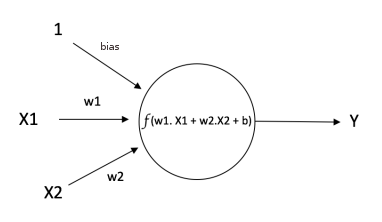
\includegraphics[width=12cm]{neuron}
	\caption{An Artificial Neuron}
	\label{fig:neuron}
\end{figure}

\begin{flushleft}
There are several different types of activation function, however every activation function takes in a single number as input and performs a certain mathematical operation on the number. The three most common activation functions generally encountered are ReLU, tanh and sigmoid. Rectified Linear Unit, or ReLU, takes in an input and replaces negative numbers with zero. The tanh function squashes the input to between the range between -1 and 1. Finally the sigmoid activation function takes the input and squashes it to the range between 0 and 1. In the field of CNN's ReLU is commonly used, as training times are significantly better when using this activation function. (\cite{krizhevsky2012imagenet}). These different types of activation function are visualised in Figure \ref{fig:functions}.
\end{flushleft}

\vspace{0.5cm}
\begin{figure}[h]
	\centering
	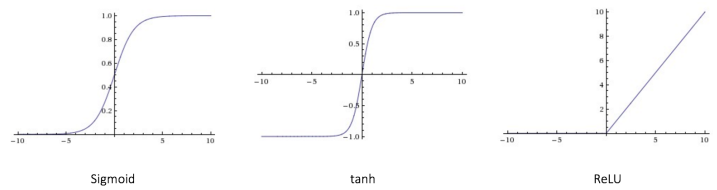
\includegraphics[width=12cm]{functions}
	\caption{Activation Functions Visualised}
	\label{fig:functions}
\end{figure}

\begin{flushleft}
A Neural Network consists of a series of interconnected layers of these artificial neurons, with the output of each layer of neurons serving as input for the next layer of neurons. The simplest and most common type of Neural Network is the feedforward neural network. It consists of multiple layers of neurons, with connections to all of the neurons in the preceding layer. Each connection or edge has a weight associated with it. There are three types of nodes - input nodes, hidden nodes and output nodes. As the name suggests, data in a feedforward neural network only moves forward through the network - into the input layer, through the hidden layers and then on to the output layer.
\end{flushleft}

\vspace{0.5cm}
\begin{figure}[h]
	\centering
	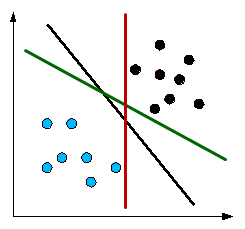
\includegraphics[width=12cm]{linear}
	\caption{Linearly Separable Data}
	\label{fig:linear}
\end{figure}

\subsection{Input Nodes}
\begin{flushleft}
Input nodes take in the input data fed into the network without performing any computation and pass the data on to the hidden nodes. These nodes make up the input layer of a neural network.
\end{flushleft}

\subsection{Hidden Nodes}
\begin{flushleft}
The hidden nodes perform the actual computation, taking data from the input nodes and providing information to the output nodes. There can be multiple or zero hidden layers in a network, whereas there will only ever be one input and output layer.
\end{flushleft}

\subsection{Output Nodes}
\begin{flushleft}
Like the input nodes, the output nodes do not perform any computation on the data - they simple take information from the hidden layers and expose this to the outside. This will generally consist of a prediction.
\end{flushleft}

\subsection{XOR Problem}
\begin{flushleft}
In the paper mentioned above, "Perceptrons: An Introduction to Computational Geometry", the Xor problem was first introduced. Xor is a function that given two binary inputs returns 0 if the inputs are equal and 1 if they are not. Xor is a classification problem with known expected results, therefore it is appropriate to utilise a Supervised Learning approach to solving it. However, the Xor problem is an example of a problem that is not linearly seperable. As mentioned previously, a single perceptron is not capable of predicting data that is not linearly seperable, therefore a single layered architecture of perceptrons is simply not capable of solving this problem. The only way for a Neural Network to solve this problem is to expand the number of layers in the architecture, adding a hidden layer. This type of architecture is known as the Multilayer Perceptron.
\end{flushleft}

\subsection{Multilayer Perceptron}
\begin{flushleft}
A Multilayer Perceptron (MLP) consists of an input layer, an output layer and one or more hidden layers, as seen in \ref{fig:mlp}. MLP's are feedforward neural networks. The MLP architecture solves the Xor problem by introducing linear seperability (\cite{Singh2016MinimumCM}).

Deep Learning is when there is more than one hidden layer present in a network (\cite{o2015introduction}). MLP's encounter issues when attempting to carry out classification tasks on large input images. As will be explained later, each pixel of an input image must correspond to an input node in the network. As every node is connected to every other node in it's preceding layer, large images quickly require a large amount of nodes in the network. A small image of size 28x28 such as the images found in the MNIST dataset will require a network with 784 input nodes. Images sourced from the Apollo dataset are of 1920x1280, which would require an input layer consisting of 2457600 nodes. This will quickly cause issues due to overfitting and network training time.

Learning takes place in a MLP through changing the connection weights for each perceptron in the network based on the error between the expected and true output of each perceptron. This is carried out through a concept known as backpropagation.
\end{flushleft}

\vspace{0.5cm}
\begin{figure}[h]
	\centering
	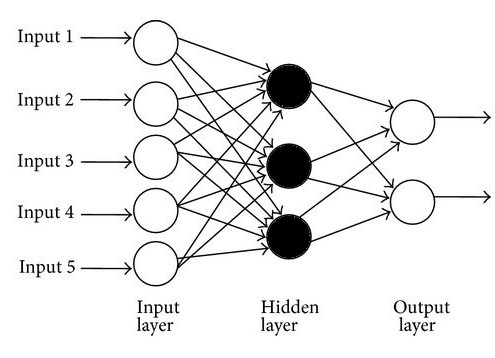
\includegraphics[width=12cm]{mlp}
	\caption{Multilayer Perceptron Architecture}
	\label{fig:mlp}
\end{figure}

\subsection{Gradient Descent and Backpropagation}
\begin{flushleft}
Gradient descent is an algorithm used to optimise the weights between neurons in such a manner that creates the least possible amount of error. When the network is training, a cost function is used to keep track of how the network is performing. The cost function looks at the discrepancies between the training output and the true values to determine an error. When the network trains, the goal is to therefore get this cost function as low as possible to ensure the lowest possible error. The way the cost function is minimised in an MLP is through gradient descent and backpropagation.

Every time the weights must be updated, the derivative of the cost function with regards to the weight itself scaled to a learning rate is subtracted. As the network trains the derivative should decrease with each training iteration. This is known as gradient descent. When the cost function cannot be reduced any more, it has converged.

The backpropagation algorithm works in conjunction with this by starting at the output layer of the network and stepping back through all the layers, updating the weights for each neuron as it goes (\cite{rumelhart1985learning}). This is in an attempt to minimise the overall error. These steps should allow the network to reduce its error and converge on an optimal solution over time as the network trains.
\end{flushleft}

\subsection{Overfitting}
\begin{flushleft}
An important point to consider when training any Machine Learning model is how well the model generalises to new data (\cite{domingos2012few}). An algorithm should be able to apply concepts learned from the training data to any previously unseen data in the problem domain in order to make accurate predictions. Overfitting is the concept of a model learning the details and noise in the training domain too well, and thus failing to provide accurate predictions on new data. Overfitting tends to occur when a model learns noise and randomness in the training data as concepts that it attempts to apply to data in the problem domain. These concepts will not apply to the new data however, and poor accuracy generally results. Although a noisy dataset will increase the severity of overfitting, it is not simply a result of a noisy dataset and can occur in any dataset (\cite{domingos2012few}). Within the field of Neural Networks, a common approach to avoid severe overfitting is to keep the network architecture relatively simple. The less parameters required to train the model, the lower the overall chance that the network will overfit and fail to generalise (\cite{o2015introduction}). However, this approach is not always feasible when dealing with large and complex datasets, and other approaches must also be taken. Another popular method to reduce overfitting is the introduction of dropout in the network. Dropout is when nodes are randomly dropped from the network along with their connections (\cite{srivastava2014dropout}). This serves to constrain the adaptation of the network while it trains in order to prevent the model from over-learning the training data.

\end{flushleft}

\section{Introduction to Machine Vision}

\begin{flushleft}
Images are represented as matrices of values, with each value corresponding to a pixel in the image. Images can be broadly broken down into two groups, grayscale and colour. A grayscale image will be represented as a 2D array of values ranging from 0 to 255, with each value representing the intensity of that pixel, as seen in Figure \ref{fig:pixels}. A value of 0 represents black and a value of 255 represents white. In grayscale images, each pixel therefore represents one colour channel (gray). In colour images however we have multiple different channels for red, green and blue. In order to represent this, a colour image will be represented as a 3D array of pixel values, with each pixel having 3 values between 0 and 255 associated with it. These three values represent the intensity of the three colour channels at that pixel. The idea is that a CNN should be able to receive these image representations as input data and return values for the probabilities of different classes.
\end{flushleft}

\vspace{0.5cm}
\begin{figure}[h]
	\centering
	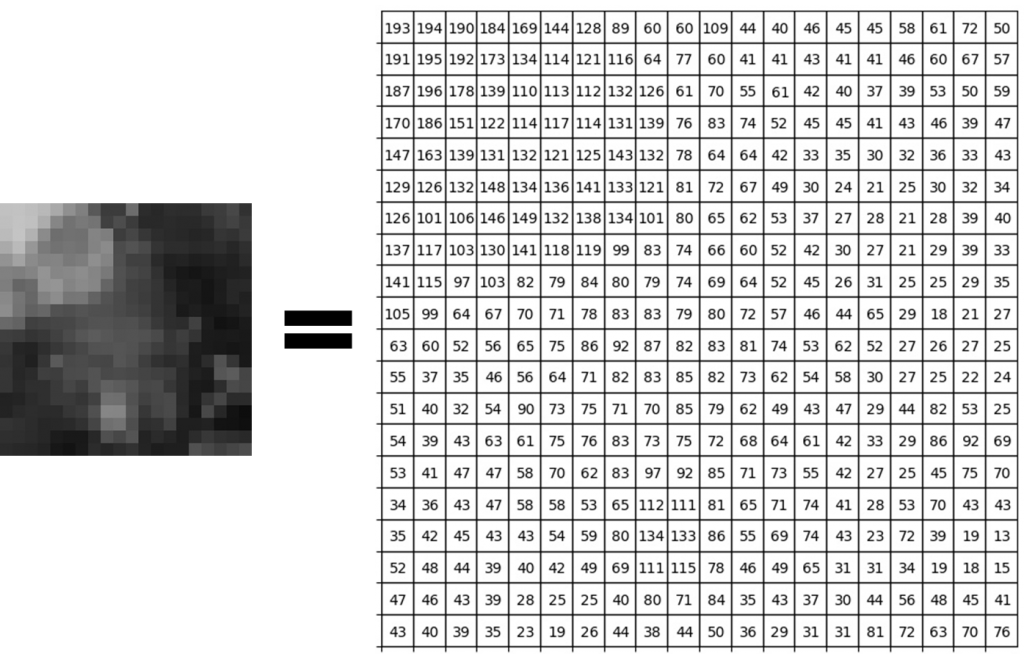
\includegraphics[width=12cm]{pixels}
	\caption{Pixel Representation of Grayscale Image}
	\label{fig:pixels}
\end{figure}

\begin{flushleft}
When humans look at an image of say, a dog, we automatically extract the features that make a dog unique in order to allow us to recognise it. For example, we may see a tail, fur and a snout and recognise that we are looking at a dog. At an extremely high level this what a CNN will do - it will look for certain low-level features such as curves and edges and build these up into more abstract concepts such as a leg or a tail in order to classify the object (\cite{lecun1995convolutional}).
\end{flushleft}

\begin{flushleft}
Interestingly enough, CNN's do take some inspiration from how the brain processes images. The visual cortex of the brain contains many fields that are sensitive to different specific elements of the input. Some groups of neurons will only respond when certain elements of the input are present, for example certain vertical edges, and other groups of neurons will respond to different elements, such as horizontal edges (\cite{youtube}). The concept of distinct groups of neurons looking for certain features is one that has translated very well into Machine Vision through the use of CNN's.
\end{flushleft}

\subsection{Edge Detection}
\begin{flushleft}
Edge detection is the ability to recognise object boundaries within an image, with most edge detection techniques using changes in pixel intensities to identify potential edges (\cite{arbelaez2011contour}). Although edge detection may appear straightforward in concept, in practice it can be a difficult task. Input images typically suffer from focal blur due to a finite point-of-field, as well as blur caused by shadows. This can cause smoothing in the variations in pixel intensity at edge points, and make it difficult to define what actually is an edge (\cite{ziou1998edge}). The magnitude of a gradient will determine if a point in the image is an edge or not - a high gradient implies that an edge is likely present. The direction of a gradient shows how the edge is oriented within the image.
\end{flushleft}

\subsubsection{Approaches}
\begin{flushleft}
There is a multitude of different techniques used for edge detection that can be split into two categories, search based and zero-crossing based. Search based techniques work by computing gradient edge strength, then searching for the direction of the edge by computing the gradient orientation. The Sobel operator, mentioned below in the explanation of the Canny edge detector, is an example of this type of technique. Zero-crossing based techniques differ in that they search for zero-crossing points on a second-order derivative function calculated from the image. Generally smooting is applied to the image prior to any of these technques (\cite{ziou1998edge}).
\end{flushleft}

\subsubsection{Canny Edge Detection}
\begin{flushleft}
Although the Canny edge detector is just one technique used for edge detection, it is one of the more prolific techniques used, and serves as a good example to illustrate the concepts used in edge detection. It consists of multiple stages. The first stage, preprocessing, involves smoothing the image to help reduce noise. Next, the gradient magnitudes and directions are calculated throughout the image via the use of the standard sobel edge detector. The magnitude of the gradient is calculated as $m=\sqrt{G_x^2+G_y^2}$ and the direction of the gradient is calculated as $0=arctan\left(\begin{array}{c}\frac{G_y}{G_x}\end{array}\right)$, where $G_x$ and $G_y$ are the derivatives of the x and y coordinates of the point under investigation. Once these are calculated the edge detection begins through the process of nonmaximum supression - if a pixel is not at maximum value it is supressed. The orientation of the pixel is placed into one of four bins representing the four possible directions the edge could be present within as illustrated in Figure \ref{fig:directions}. The possible edge directions at the grey pixel point could be either north to south (represented by the green pixels), east to west (represented by the blue pixels) or one of the diagonal directions (represented by the yellow and red pixels). Nonmaximum suppression is then applied to these four different possible areas. If the gradient orientation is at a value such as the one represented in Figure \ref{fig:orientation}, then the edge is moving diagonally perpendicular to the gradient direction. To check if a pixel belongs to an edge, its value is checked against its neighbours along the same orientation to see if the gradient is maximum and if it is above a defined threshold. If so, the pixel is marked as an edge. After this process of nonmaximum suppression, thin edges that may be broken at points are left. An edge thresholding process called hysteresis is used to fill in these broken points (\cite{canny1986computational}). Hysteresis counters the "streaking" effect of broken lines by setting both an upper and lower threshold for pixel gradient magnitudes. Values above the upper limit are accepted and values below the lower limit are rejected. Values which lie between the two limits are accepted if they lie between two points above the upper limit, reducing the overall gaps exhibited in the line. An example of Canny edge detection being used in a road environment is shown in Figure \ref{fig:canny}.
\end{flushleft}

\newpage
\vspace{0.5cm}
\begin{figure}[h]
	\centering
	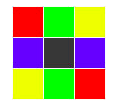
\includegraphics[width=8cm]{directions}
	\caption{Possible Edge Directions}
	\label{fig:directions}
\end{figure}

\newpage
\vspace{0.5cm}
\begin{figure}[h]
	\centering
	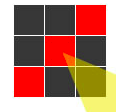
\includegraphics[width=8cm]{orientation}
	\caption{Orientation Value}
	\label{fig:orientation}
\end{figure}

\vspace{0.5cm}
\begin{figure}[h]
	\centering
	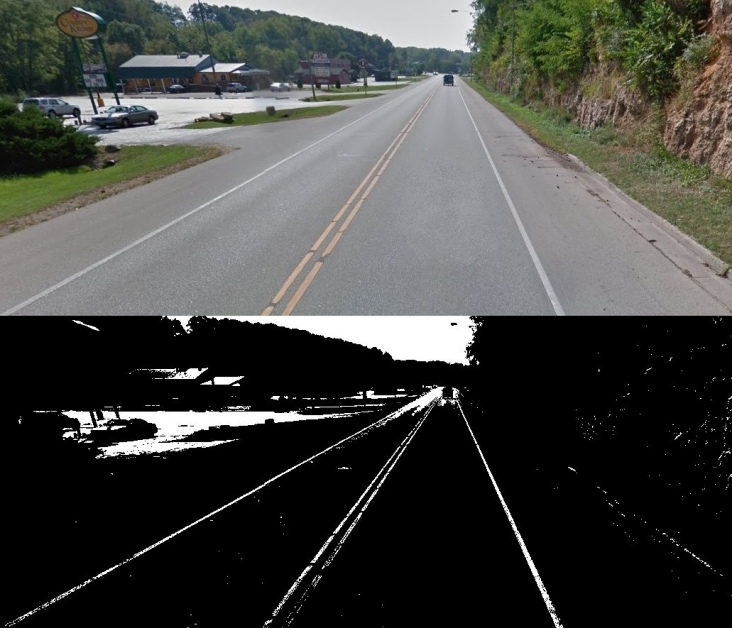
\includegraphics[width=12cm]{canny}
	\caption{Canny Edge Detection}
	\label{fig:canny}
\end{figure}

\section{Introduction to Convolutional Neural Networks}
\begin{flushleft}
Convolutional Neural Networks have recently become the standard Neural Network used within the field of image-based Machine Learning tasks (\cite{o2015introduction}). They follow essentially the same architecture as a standard Multi Layer Perceptron, except that they include extra layers of Convolution and Pooling. When these layers of Convolution and Pooling are stacked with the Fully-Connected layers of the MLP, a CNN architecture has been formed. Once Convolution and Pooling has been performed the fully-connected layer will compute the overall class scores, resulting in a final output of 1x1xn, where n is the number of possible classes.
\end{flushleft}

\vspace{0.5cm}
\begin{figure}[h]
	\centering
	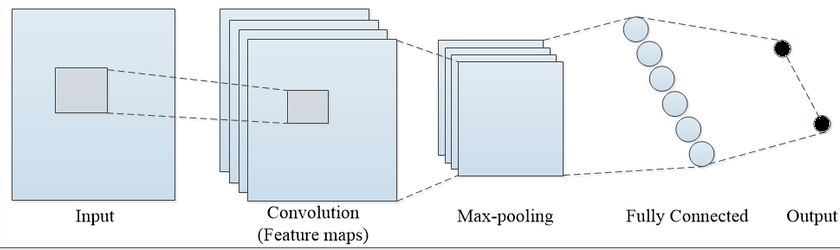
\includegraphics[width=12cm]{convo}
	\caption{CNN Architecture}
	\label{fig:convo}
\end{figure}

\newpage
\subsection{Convolution Layer}
\begin{flushleft}
There are three important points of note regarding the Convolution layer: the input image, the feature detector and the feature map. The input image is the image which the CNN is given. The feature detector is a matrix (usually 3x3 or 7x7), also called the kernel or filter, which is multiplied with the matrix values of the input image to create the feature map. The aim of this is to capture important features of the image, maintaining these important features while losing some unimportant elements and reducing overall image size. The way this works is the feature detector slides over the whole image. The particular point on the image that the feature detector is over is known as the receptive field. The parameter known as the stride is the value of the number of pixels by which the feature detector slides over the input image. For example, a stride of 2 will slide the feature detector over the input image jumping 2 pixels at a time. As the feature detector slides around the input image, the pixel values of the feature detector are multiplied against the pixel values of the input image. These multiplications are all summed to give a single value, as shown in Figure \ref{fig:conv}. The higher the value, the higher the likelihood that the particular feature represented in the feature detector is present in that section of the input image. The feature detector then slides on to carry out this process for every section of the input image.
\end{flushleft}

\vspace{0.5cm}
\begin{figure}[h]
	\centering
	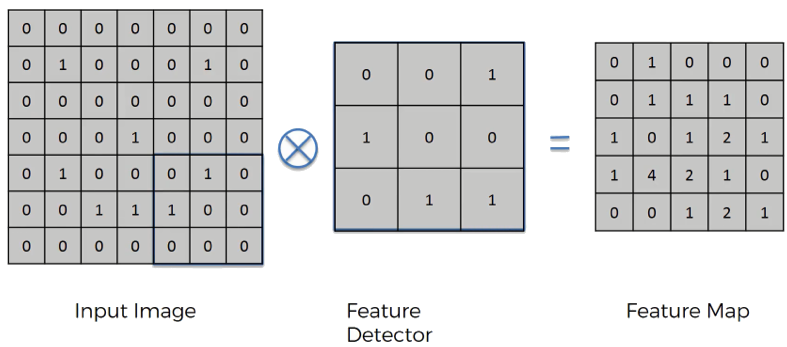
\includegraphics[width=12cm]{conv}
	\caption{Convolution Layer}
	\label{fig:conv}
\end{figure}

\newpage
\subsection{Pooling Layer}
\begin{flushleft}
The pooling layer performs downsampling to extract key important features and reducing the number of parameters. The pooling layer operates over every feature map and by pacing a matrix over the feature map and selecting the min value, max value or mean value, depending on the type of pooling being utilised, as shown in Figure \ref{fig:pool}. These extracted values form the pooled feature map. Pooling helps to reduce image size while also extracting important features.
\end{flushleft}

\vspace{0.5cm}
\begin{figure}[h]
	\centering
	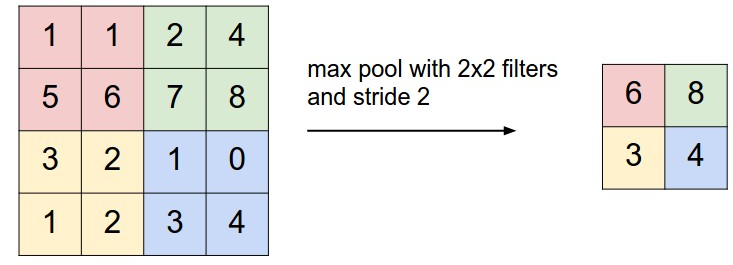
\includegraphics[width=12cm]{pool}
	\caption{Pooling Layer}
	\label{fig:pool}
\end{figure}

\newpage
\subsection{Evaluating the Classifier}
\begin{flushleft}
There are various techniques which can be used to evaluate the operation of a classifier. Some of the more prevalent ones, many of which will be seen throughout the rest of this report, are explained below.
\end{flushleft}

\subsubsection{Top-1 and Top-5 Accuracy}
\begin{flushleft}
First, the CNN makes a classification. Then in the case of Top-1, the class of the highest probability is checked against the target label. In the case of Top-5, the target label is compared with the top five highest probability predictions. Following this, in both cases the classifier score is calculated as the number of times that the prediction matched in either Top-1 or Top-5, divided by the total number of data points.
\end{flushleft}

\subsubsection{Accuracy Issues}

\begin{flushleft}
Generally speaking using accuracy alone (number of correctly labelled classes) is not a very reliable metric for an object detection classifer. For example, if there were 95 dogs and 5 cats to be classified a classifier may label all objects present as dogs. This would lead to an overall accuracy score of 95\%, however this classifier is obviously quite flawed. This is known as class imbalance, and in real life scenarios tends to be the norm. The decisions reached by the classifier can be explained as follows:

\begin{enumerate}
  \item True positive: a positive example classified as positive
  \item True negative: a negative example classified as negative
  \item False positive: a negative example classified as positive
  \item False negative: a positive example classified as negative
\end{enumerate}

False negatives are particularly an issue for the field of self-driving cars, where this result could have potentially fatal ramifications. An example of a false negative classification was seen during a fatal crash of a Tesla model S in May 2016, whereby the autopilot system failed to recognise a white truck against a clear, brightly lit sky. Thus, we need to do more than just measure accuracy in order to properly evaluate the classifier (\cite{rogers2016first}).
\end{flushleft}

\subsubsection{Confusion Matrix}
\begin{flushleft}
A Confusion Matrix, also referred to as an Error Matrix, is a relatively simple technique for classifier evaluation. It is essentially a table that plots the number of correct and incorrect predictions for all of the different classes. The false positives, false negatives, true positives and true negatives are plotted then the average value for all classes combined is calculated, as demonstrated in the confusion matrix below.

\begin{table}[]
\begin{tabular}{lllllll}
          &                        & \multicolumn{1}{r}{Actual}           &                                      &  &  &  \\
          &                        & \multicolumn{1}{c}{+}                & \multicolumn{1}{c}{-}                &  &  &  \\ \cline{3-4}
Predicted & \multicolumn{1}{l|}{Y} & \multicolumn{1}{l|}{True Positives}  & \multicolumn{1}{l|}{False Positives} &  &  &  \\ \cline{3-4}
          & \multicolumn{1}{l|}{N} & \multicolumn{1}{l|}{False Negatives} & \multicolumn{1}{l|}{True Negatives}  &  &  &  \\ \cline{3-4}
          &                        &                                      &                                      &  &  &  \\
          &                        &                                      &                                      &  &  & 
\end{tabular}
\end{table}
\end{flushleft}

\subsubsection{Other Evaluation Metrics}
\begin{flushleft}
There are a number of different metrics of evaluation that can be used other than accuracy alone, with the major ones being summarised in the section. An important point to note is that each of these metrics is derived from the confusion matrix explained above, and can be thought of as different ways of summarising the matrix.

\vspace{0.5cm}
\textbf{Precision}
\linebreak
The precision is the number of correct positive predictions compared to the actual number of positive examples. It can be represented by the formula $precision = \frac{\#TP}{\#TP + \#FP}$. This is a good metric to evaluate when there is a high cost associated with a false positive. For example, an email spam detector must have high precision in order to avoid mistakenly classifying legitimate emails as spam. 

\vspace{0.5cm}
\textbf{Recall}
\linebreak
The recall is the ratio of correct positive examples to the number of positive predictions, and can be represented as $recall = \frac{\#TP}{\#TP + \#FN}$. Recall is an important metric when there is a high cost associated with false negatives and as mentioned above are an extremely important metric for this project.

\vspace{0.5cm}
\textbf{F-score}
\linebreak
Another metric can be derived from precision and recall, known as F-score. F-score is the harmonic mean of precision and recall, and is defined as 
$F = 2. \frac{precision - recall}{precision + recall}$. The F-score can be thought of as representing the balance between the precision and the recall. Although this is an important metric overall, it does not take precedence in this project, where a good recall score is of utmost importance.
\end{flushleft}

\subsubsection{AUC-ROC Curve}
\begin{flushleft}
The AUC (Area Under Curve) ROC (Receiver Operating Characteristics) curve is another method of classifier evaluation, enabling the visualisation of results from a classification problem. The ROC curve is used to plot the true positve rate against the false positive rate, resulting in a probability curve, while the AUC represents how well the model distinguishes between classes. The higher the AUC, the better the model is. This is visualised in Fig \ref{fig:aucroc}.
\end{flushleft}

\vspace{0.5cm}
\begin{figure}[h]
	\centering
	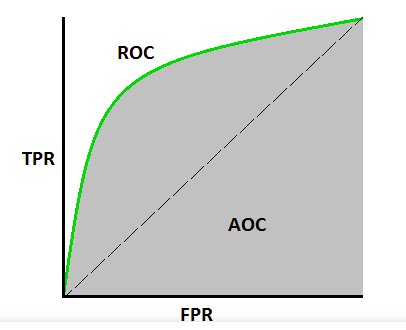
\includegraphics[width=12cm]{aucroc}
	\caption{AUC-ROC Visualised}
	\label{fig:aucroc}
\end{figure}

\newpage
\section{Tensorflow Introduction}

This section is dedicated to the background work done in order to gain an understanding of how to implement CNN's using tensorflow. The experiments illustrated in this section were carried out during the completion of the Complete Guide to TensorFlow for Deep Learning with Python course on Udemy (\cite{udemy}). This section consists of two experiments carried out on the MNIST and CIFAR-10 datasets. The first experiment is sample code provided as part of the course to illustrate the concepts learned during the course. The second experiment is an exercise for the course carried out to implement an understanding of these concepts.

\subsection{MNIST Experiment}

The first experiment carried out was the implementation of a very simple CNN. The architecture of the CNN consisted of two layers of Convolution, two pooling layers and a fully-connected layer. After carrying out 5000 training steps with a batch size of 50, a final Top-1 accuracy of 98.75\% was achieved.

\subsubsection{Code Breakdown}

\begin{flushleft}
The functions displayed in Figure \ref{fig:helpers} are all helper functions. The init\_weights function initialises the random weights for fully connected or convolution layers, with the shaper of the layer passed in as a parameter. The init\_bias function performs the same operation for the bias. The conv2d function creates a convolution using a built in function from tensorflow. The max\_pool\_2by2 function creates a max pooling layer, also using built in tensorflow functions. The convolutional\_layer function uses the conv2d function to return an actual convolutional layer with a ReLu activation function. Lastly, the normal\_full\_layer returns a normal fully connected layer.
\end{flushleft}

\vspace{0.5cm}
\begin{figure}[h]
	\centering
	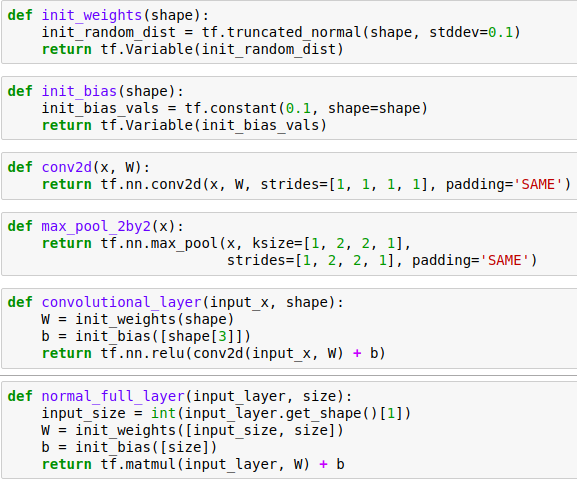
\includegraphics[width=12cm]{helpers}
	\caption{Creating Helper Functions}
	\label{fig:helpers}
\end{figure}

\begin{flushleft}
The functions displayed in Figure \ref{fig:layers} are used to create the convolution and pooling layers of the network. In creating convo\_1, we can see that a 6x6 filter is used from the parameters. An ouput value of 32 is used to represent the number of filters used. The parameter of 1 represents the original input of the image. This carries down to the other layers, with convo\_2 taking in an input image of 32 from convo\_1.
\end{flushleft}

\vspace{0.5cm}
\begin{figure}[h]
	\centering
	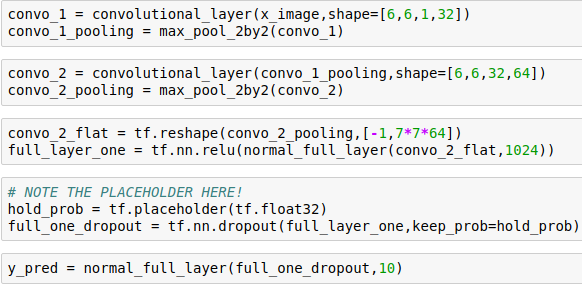
\includegraphics[width=12cm]{layers}
	\caption{Creating Layers}
	\label{fig:layers}
\end{figure}

\begin{flushleft}
The code displayed in Figure \ref{fig:training} shows the model being trained. A tensorflow session is created and data is read in from the dataset. The session is ran to begin model training. The current training step and current error calculated from a loss function is displayed as output as the model trains.
\end{flushleft}

\vspace{0.5cm}
\begin{figure}[h]
	\centering
	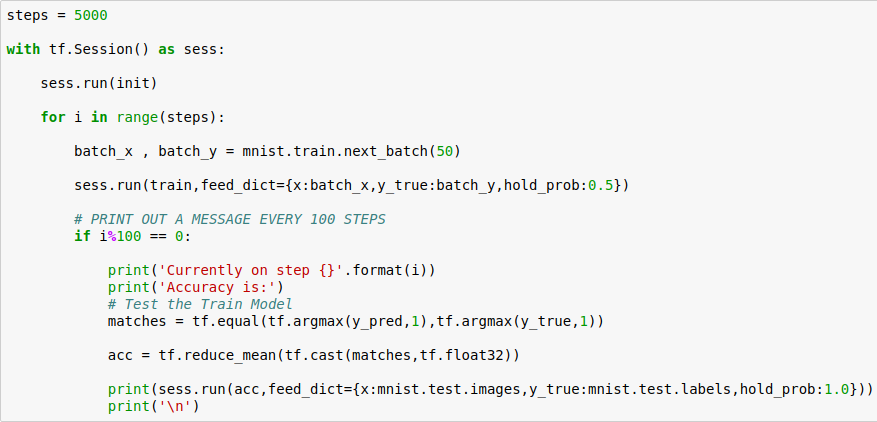
\includegraphics[width=12cm]{training}
	\caption{Training the Model}
	\label{fig:training}
\end{figure}

\newpage
\subsection{CIFAR-10 Experiment}

\begin{flushleft}
The second experiment was carried out on the CIFAR-10 dataset, and the architecture used was consistent with the first experiment, consisting of two layers of Convolution and Pooling. After 5000 training steps with a batch size of 100, a final Top-1 accuracy of 72\% was reached.
\end{flushleft}

\subsection{Initial Findings}

The first two experiments were carried out using CNN's of the same architecture, however an accuracy discrepancy of 26.75\% was observed. Both datasets contain images labelled into 10 classes. The differences arise in the dataset size and image complexity. Firstly, the CIFAR-10 dataset contains 50,000 training images, whereas the MNSIT dataset contains 60,000 training images. The images in the MNSIT dataset are grayscale, whereas images in the CIFAR-10 dataset consist of 3 colour channels. The images in the CIFAR-10 dataset are also of a higher complexity compared to the handwritten digits in the MNIST dataset. The CIFAR-10 images contain more complex real-world images with noisy backgrounds. These disprepancies between the datasets may explain the disprepancies in the accuracy achieved by the classifiers.

\subsection{Experiment Environments}
\begin{flushleft}
Initial environment setup to carry out the below experiments proved quite challenging. During the first attempts at carrying out the experiments, tensorflow was erroneously installed to run using the training machines CPU. This lead to untenable training times for the experiments. Although the training times were not recorded precisely, each experiment took over a day to finish training, during which time the training machine was rendered essentially unusable due to the high load on its CPU. There were two main take-aways from the initial iterations:

\begin{enumerate}
  \item Tensorflow should be installed properly to use the GPU in order to manage training times.
  \item Training times should be recorded for better understanding of the experiments.
\end{enumerate}

\end{flushleft}

\subsubsection{Tensorflow Install}
\begin{flushleft}
The initial attempts to setup tensorflow were carried out on a machine running Windows 7. Several versioning issues were encountered due to Bazel, the build tool used to compile tensorflow. These issues were solved via downgrading to an earlier version of Bazel, however new versioning issues were then encountered due to CUDNN, Nvidias GPU-accelerated library for deep learning. Several different versions were installed without success. Due to these issues seemingly being exclusive to Windows, it was decided to attempt an install on a different machine running Ubuntu. The tensorflow install for the Ubuntu machine was carried out without issue. All neccessary Nvidia drivers were installed on the system, and tensorflow was then installed and the experiments were rerun. The training times for running the two experiments with GPU acceleration were 12 and 16 minutes respectively, a vast improvement over the initial times. The GPU on the Ubuntu machine was an Nvidia Geforce GTX 650 with 2GB memory.
\end{flushleft}

\subsubsection{Memory Issues}
\begin{flushleft}
Although the first two experiments ran without issues, problems were quickly encountered when modifications were made to the Cifar-10 experiment. In an attempt to improve accuracy results, two further layers of convolution and pooling were added. This led the out of memory (OOM) errors being thrown during training. This was caused by the graphical memory on the training machine being maxed out at the full 2GB. After extensive research around this area several attempts at rectifying the issues were carried out. The first attempt tried was reduction of batch size from 100 images, causing less of the dataset being loaded into memory. At a batch size of 4 images, the three layer network successfully trained. The issue with this approach however is that a smaller batch size causes the gradient estimate of the network to be less accurate, and Top-1 accuracy of the network dropped to 60.46\%. The second approach was to simply keep the number of layers low, resulting in a simpler network with less memory requirements. Both of these solutions were not viable for this project. Poor accuracy scores and an inability to train complex networks created an obvious demand for a more powerful training machine. Another point to note is image size disparities between the Cifar-10 dataset and the overall target dataset for this project, the Apollo self-driving car image dataset. A machine struggling with the 32x32 low resolution images of the Cifar-10 dataset would surely run into a host of issues with the 1920x1080 images of the target dataset. As such, it was decided that a much more advanced machine would be required. It was decided that Amazon Web Services (AWS) was the only way to quickly and easily access the required computational power demanded by this project.
\end{flushleft}

\subsubsection{AWS Setup}
\begin{flushleft}
One of the many services offered by the AWS platform is Amazon Machine Images (AMI) for Deep Learning. These are virtual machine instances that launch with pre-installed pip deep learning frameworks such as tensorflow, keras etc. in different environments, as well as GPU acceleration. This allows development of models remotely from a client machine which can be then trained using the available GPU resources on the deep learning instance. These instances can be deployed and the desired environment (tensorflow in this case) activated. Jupyter notebooks can be run as normal on the AWS instance, and a rule is set up on the client machine to forward all requests on a certain port to the AWS instance. This allows the user to write code in a Jupyter notebook remotely on the AWS instance. The instance type chosen for this project was the p2.xlarge instance which contains 122GiB of memory, 16 virtual CPU cores and a Nvidia K80 GPU. The steps followed was from the official AWS documentation.
\end{flushleft}

\subsubsection{Cifar-10 Further Experiments}
\begin{flushleft}
As mentioned above, further experiments were carried out on the Cifar-10 dataset in an attempt to improve the disappointing initial results. The base code provided as part of the tutorial (\cite{udemy}) was modified in a range of different ways in order to maximise results. In order to evaluate the network properly the following metrics were recorded:

\begin{enumerate}
  \item Peak Top-1 accuracy
  \item Precision
  \item Recall
  \item Training time
\end{enumerate}

The baseline of these metrics achieved by the simple network provided from the tutorial are shown in the table below, with the accuracy, precision and recall being graphed in Fig \ref{fig:baseline}. Interestingly enough, the accuracy and recall values for this experiment were identical throughout all of the training steps. This does not necessarily mean that there is an issue, however it is very unusual. A focus for the following experiments was to investigate what changes, if any, would cause these values to diverge.
\end{flushleft}

\vspace{0.5cm}
\begin{tabular}{llll}
                                          & Initial Experiment                 &                                &                              \\ \hline
\multicolumn{1}{|l|}{Peak Top-1 accuracy} & \multicolumn{1}{l|}{Training Time} & \multicolumn{1}{l|}{Precision} & \multicolumn{1}{l|}{Recall}  \\ \hline
\multicolumn{1}{|l|}{70.16\%}             & \multicolumn{1}{l|}{220s}          & \multicolumn{1}{l|}{71.67\%}   & \multicolumn{1}{l|}{70.16\%} \\ \hline
\end{tabular}

\vspace{0.5cm}
\begin{figure}[h]
	\centering
	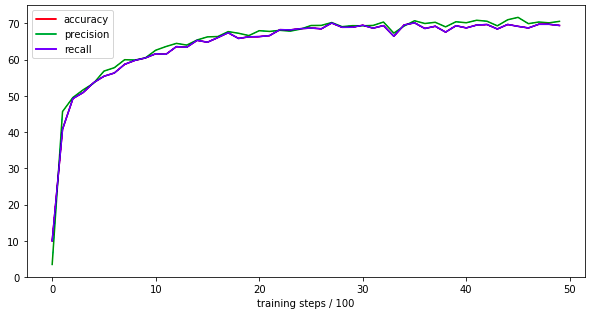
\includegraphics[width=12cm]{baseline-graph}
	\caption{Baseline Plot}
	\label{fig:baseline}
\end{figure}

\begin{flushleft}
\vspace{0.5cm}
\textbf{Experiment 1: Training Steps}
\linebreak
Before investigating the effects of altering the network architecture, the optimal number of training steps was investigated. This parameter was investigated first as it has a large effect on training time. A network that does not have enough training steps will underlearn, whereby it does not learn all possible parameters. However having too many training steps will lead to increased training time with no increase in accuracy. The initial experiment carried out 5000 training steps, so this was doubled to 10,000 steps in an attempt to see if this would boost accuracy, precision and recall. The results are displayed in the table below and plotted in Fig \ref{fig:experiment-1}. All three metrics levelled off at around the 5000 step mark, with no significant increases reported. It would therefore appear that 5000 training steps is the optimal value.

\vspace{0.5cm}
\begin{tabular}{llll}
                                           & Experiment 1                       &                                                             \\ \hline
\multicolumn{1}{|l|}{Peak Top-1 accuracy} & \multicolumn{1}{l|}{Training Time} & \multicolumn{1}{l|}{Precision} & \multicolumn{1}{l|}{Recall}  \\ \hline
\multicolumn{1}{|l|}{70.46\%}             & \multicolumn{1}{l|}{466s}          & \multicolumn{1}{l|}{70.71\%}   & \multicolumn{1}{l|}{70.46\%} \\ \hline
\end{tabular}

\vspace{0.5cm}
\begin{figure}[h]
	\centering
	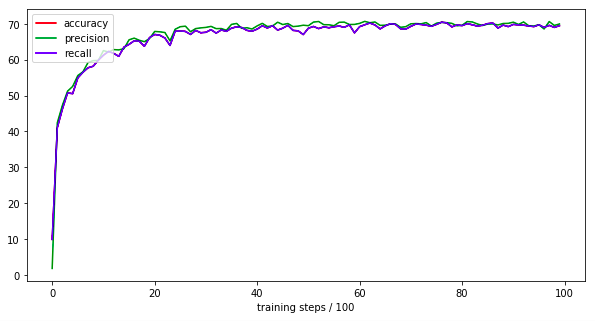
\includegraphics[width=12cm]{experiment-1}
	\caption{10,000 Training Steps}
	\label{fig:experiment-1}
\end{figure}
\end{flushleft}

\begin{flushleft}
\vspace{0.5cm}
\textbf{Experiment 2: Convolution and Pooling Layers}
\linebreak
The next experiment undertaken was to increase the number of convolution and pooling layers. For this experiment only one extra layer of convolution and pooling was added. As can be shown in the results displayed in the table below as well in Fig \ref{fig:experiment-2}, this did not yield any significant results.

\vspace{0.5cm}
\begin{tabular}{llll}
                                          & Experiment 2                       &                                &                              \\ \hline
\multicolumn{1}{|l|}{Peak Top-1 accuracy} & \multicolumn{1}{l|}{Training Time} & \multicolumn{1}{l|}{Precision} & \multicolumn{1}{l|}{Recall}  \\ \hline
\multicolumn{1}{|l|}{70.38\%}             & \multicolumn{1}{l|}{192s}          & \multicolumn{1}{l|}{70.82\%}   & \multicolumn{1}{l|}{70.38\%} \\ \hline
\end{tabular}

\vspace{0.5cm}
\begin{figure}[h]
	\centering
	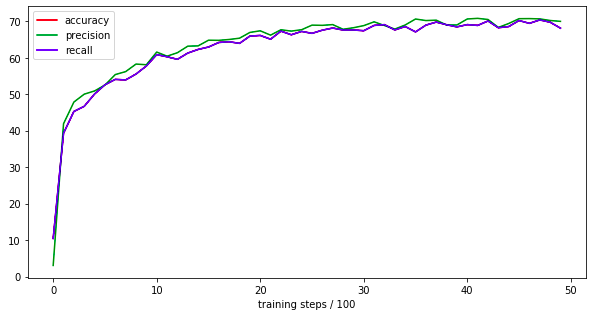
\includegraphics[width=12cm]{experiment-2}
	\caption{Experiment 2}
	\label{fig:experiment-2}
\end{figure}
\end{flushleft}

\begin{flushleft}
\vspace{0.5cm}
\textbf{Experiment 3: Fully Connected Layers}
\linebreak
As the extra layers of convolution and pooling had failed to yield any benefits, the next step taken was to increase the number of fully connected layers in the network. One extra fully connected layer was added as well as a dropout layer. The reasoning behind this experiment was to investigate the possibility that the network was performing poorly with the class predictions. The images in the Cifar-10 dataset consist of non-occluded blurred objects with one class of object present per image. As such it was reasoned that only a small number of convolution and pooling layers were required to extract feature maps from the images, and increased numbers of fully-connected layers would be more important. Dissapointingly, the results of this experiment were a marginal drop in accuracy, precision and recall.

\vspace{0.5cm}
\begin{tabular}{llll}
                                          & Experiment 3                       &                                &                              \\ \hline
\multicolumn{1}{|l|}{Peak Top-1 accuracy} & \multicolumn{1}{l|}{Training Time} & \multicolumn{1}{l|}{Precision} & \multicolumn{1}{l|}{Recall}  \\ \hline
\multicolumn{1}{|l|}{69.52\%}             & \multicolumn{1}{l|}{161s}          & \multicolumn{1}{l|}{69.67\%}   & \multicolumn{1}{l|}{69.52\%} \\ \hline
\end{tabular}

\vspace{0.5cm}
\begin{figure}[h]
	\centering
	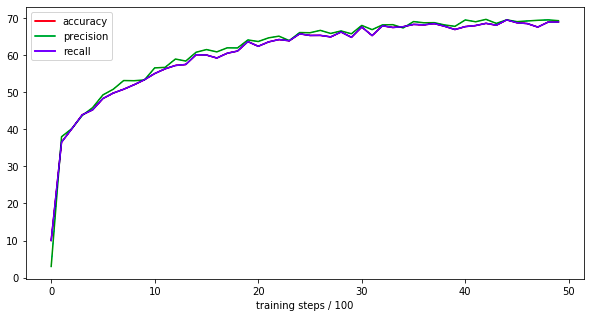
\includegraphics[width=12cm]{experiment-3}
	\caption{Experiment 3}
	\label{fig:experiment-3}
\end{figure}
\end{flushleft}

\newpage
\begin{flushleft}
\vspace{0.5cm}
\textbf{Experiment 4: Convolution, Pooling and Fully Connected Layers}
\linebreak
As Experiments 3 and 4 had failed to yield better results, 2 extra layers of convolution and pooling were added in conjunction with an extra fully-connected layer. As can be seen from the results table and Fig \ref{fig:experiment-4}, results actually went down marginally.

\vspace{0.5cm}
\begin{tabular}{llll}
                                          & \multicolumn{1}{c}{Experiment 4}   &                                &                             \\ \hline
\multicolumn{1}{|l|}{Peak Top-1 accuracy} & \multicolumn{1}{l|}{Training Time} & \multicolumn{1}{l|}{Precision} & \multicolumn{1}{l|}{Recall} \\ \hline
\multicolumn{1}{|l|}{67.3\%}              & \multicolumn{1}{l|}{276s}          & \multicolumn{1}{l|}{68.56\%}   & \multicolumn{1}{l|}{67.3\%} \\ \hline
\end{tabular}

\vspace{0.5cm}
\begin{figure}[h]
	\centering
	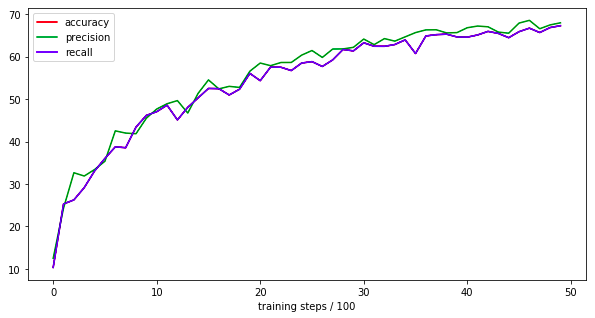
\includegraphics[width=12cm]{experiment-4}
	\caption{Experiment 4}
	\label{fig:experiment-4}
\end{figure}
\end{flushleft}

\newpage
\begin{flushleft}
\vspace{0.5cm}
\textbf{Experiment 5: Extra Dropout Layers}
\linebreak
Following the failure of experiment 4 to improve results, 2 extra layers of dropout with a probability of 0.25 were added to the experiment 4 architecture after the 2nd and 4th pooling layers in an attempt to tale any potential overfitting. Dropout is not typically implemented in modern convolutional networks, however as the purpose of these experiments is purely to investigate the effects of different techniques it was implemented for this experiment. Although the results summarised in the table below and Fig \ref{fig:experiment-5} do not show any meaningful increase in accuracy either, the accuracy curve from this experiment as well as experiment 4 suggest that the network is underlearning as the curves do not level off as much as in previous results. This implied that the network may simply need more time to train. Interestingly, during this experiment the accuracy and recall metrics diverged from one another, as can be oserved in Fig \ref{fig:experiment-5}. This would seem to imply that the network may have been overfitting slightly.

\vspace{0.5cm}
\begin{tabular}{llll}
                                          & \multicolumn{1}{c}{Experiment 5}   &                                &                              \\ \hline
\multicolumn{1}{|l|}{Peak Top-1 accuracy} & \multicolumn{1}{l|}{Training Time} & \multicolumn{1}{l|}{Precision} & \multicolumn{1}{l|}{Recall}  \\ \hline
\multicolumn{1}{|l|}{60.47\%}             & \multicolumn{1}{l|}{425s}          & \multicolumn{1}{l|}{60.60\%}   & \multicolumn{1}{l|}{60.57\%} \\ \hline
\end{tabular}

\vspace{0.5cm}
\begin{figure}[h]
	\centering
	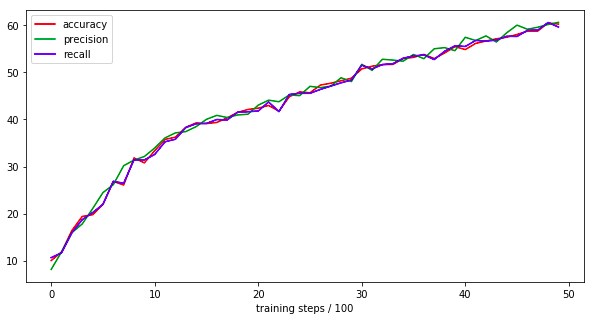
\includegraphics[width=12cm]{experiment-5}
	\caption{Experiment 5}
	\label{fig:experiment-5}
\end{figure}
\end{flushleft}

\newpage
\begin{flushleft}
\vspace{0.5cm}
\textbf{Experiment 6: Increased Training Steps}
\linebreak
The observations in experiments 4 and 5 suggested that the network might simply need more time to train. In experiment 1 it was concluded that 5000 training steps would be sufficient, however this experiment was carried out using the simple baseline network architecture. It was therefore a mistake to assume that 5000 training steps would be sufficient for all following experiments. The number of training steps was increased drastically to 25,000, with the architecture remaining the same as in experiment 5. Although training time was significantly increased, all metrics gained a slight increase with accuracy peaking at 73.25\%, a decent improvement from the initial results.

\vspace{0.5cm}
\begin{tabular}{llll}
                                          & \multicolumn{1}{c}{Experiment 6}   &                                &                              \\ \hline
\multicolumn{1}{|l|}{Peak Top-1 accuracy} & \multicolumn{1}{l|}{Training Time} & \multicolumn{1}{l|}{Precision} & \multicolumn{1}{l|}{Recall}  \\ \hline
\multicolumn{1}{|l|}{73.54\%}             & \multicolumn{1}{l|}{1778s}         & \multicolumn{1}{l|}{74.03\%}   & \multicolumn{1}{l|}{73.48\%} \\ \hline
\end{tabular}

\vspace{0.5cm}
\begin{figure}[h]
	\centering
	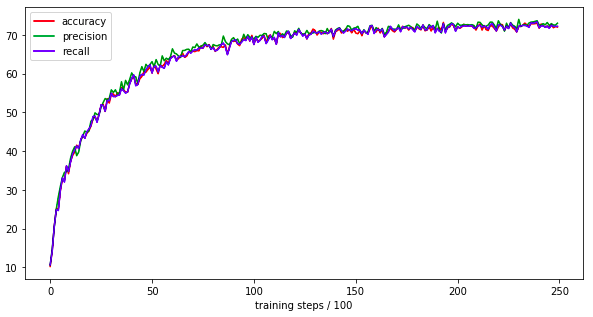
\includegraphics[width=12cm]{experiment-6}
	\caption{Experiment 6}
	\label{fig:experiment-6}
\end{figure}

\end{flushleft}

\newpage
\vspace{0.5cm}
\textbf{Confusion Matrix}
\linebreak
The confusion matrix is outlined in Fig \ref{fig:cm}.

\vspace{0.5cm}
\begin{figure}[h]
	\centering
	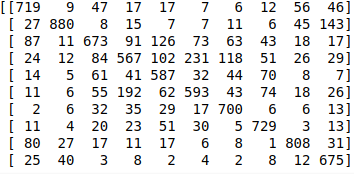
\includegraphics[width=12cm]{cm}
	\caption{Confusion matrix}
	\label{fig:cm}
\end{figure} 

\begin{flushleft}
\vspace{0.5cm}
\textbf{Conclusions}
\linebreak
These experiments conclude with a small yet significant increase in accuracy, precision and recall scores from the final experiment. Adding just extra layers of convolution and pooling without adding extra fully-connected layers did not result in improvements, and vice versa. Upon creation of a more complex network architecture with dropout layers results actually went down slightly. However, observation of the metric graphs showed that the network was possibly underlearning, and a drastic increase in training steps led to positive results. Accuracy, precision and recall all seemed to increase in proportion with one another for these experiments, however this is generally not guaranteed for all networks. Datasets containing more classes or high levels of class imbalance would typically not result in such regular accuracy, precision and recall metrics. If there is anything to take from these experiments moving forward with this project, it is that simply adding one or two extra layers is not sufficient to gain satisfactory results - adding multiple layers of convolution, pooling and fully-connected layers should be investigated in conjunction with each other in future experiments. As the unusual accuracy and recall results also demonstrate, it may also be beneficial to introduce dropout or some other form of regularisation in networks that are not obviously overfitting. Although the increases in performance shown are slight, I am confident that further increasing the complexity of the network and increasing training times can lead to further increases.

\end{flushleft}

\newpage
\chapter{Empirical Studies}
\begin{flushleft}
The following sections will investigate the effects of retraining various different network architectures using transfer learning, as well as investigate the effects of parameter tuning upon these networks. Transfer learning is a popular technique in Machine Learning whereby an already trained model is applied to new data. As mentioned earlier, CNN's use their lower layers to extract primitive features such as edges, the middle layers detect shapes from these edges and the final layers learn the task specific abstractions of these shapes. In transfer learning the last layers of the network are retrained using data from the target domain, allowing the insights that have been learned from the original data to be applied to the new data. This helps to avoid training models from scratch on unseen yet related datasets. Transfer learning is a very popular field within Machine Learning, as it can help drastically cut down on training times, as well as enabling better results on smaller datasets.
\end{flushleft}
\section{Inception V3 Retraining}

\newpage
\chapter{Classifier Implementation}
\section{Requirements}
\section{System Design}
\section{Implementation}
\section{Analysis}

\newpage
\chapter{Final Conclusion}
\section{Review of Research}
\section{Reflections on Implementation}

\printbibliography

\end{document}